\documentclass[pdftex,12pt,fullpage,oneside]{amsart}
\usepackage{array,amsmath,psfrag,amssymb,subfigure,tabularx}
\usepackage{hyperref,multicol}
\usepackage{booktabs}
\usepackage{vmargin,boxedminipage}
\usepackage[usenames]{color}
\usepackage{datetime}
\usepackage{dcolumn}
\usepackage{wrapfig}
\usepackage{setspace}
\usepackage{url}
\usepackage[english]{babel}
\usepackage{times}
\usepackage{multirow}
\usepackage{multicol}
\usepackage[pdftex]{graphicx}
\usepackage{lscape}
\usepackage{multicol}
\usepackage[top=2in,right=0in,left=2in,bottom=1in]{geometry}
\usepackage{array}
\usepackage{dcolumn}
\usepackage{booktabs}
\usepackage{hyperref}
\graphicspath{{graphics/}}

%\usepackage[authoryear,sort&compress]{natbib}
\usepackage{natbib}
\bibpunct{(}{)}{;}{a}{}{,}
%\bibdata{/Users/jacobmontgomery/Dissertation/master3}
\bibdata{flo_Bib,/Users/jacobmontgomery/Dissertation/master3}


\title{Dynamic Conflict Forecast - Improving Conflict Predictions
  Using Ensemble Bayesian Model Averaging}\thanks{This project was undertaken in the
  framework of an initiative funded by the Information Processing
  Technology Office of the Defense Advanced Research Projects Agency
  aimed at producing models to provide an Integrated Crisis Early
  Warning Systems (ICEWS) for decision makers in the U.S. defense
  community. The holding grant is to the Lockheed Martin Corporation,
  Contract FA8650-07-C-7749. All the bad ideas and mistakes are our
  own.}  
 
\author[M.D. Ward]{Michael D. Ward}
\address{Professor M.D. Ward, Department of Political Science,
Duke University, Durham, NC, USA, 27708}
\email{\url{michael.d.ward@duke.edu}}

\author[J. M. Montgomery]{Jacob M. Montgomery}
\address{Jacob M. Montgomery, Department of Political Science,
Duke University, Durham, NC, USA, 27708 }
\email{\url{jacob.montgomery@duke.edu}}

  \author[F. M.  Hollenbach]{Florian M. Hollenbach}
\address{Florian M. Hollenbach, Department of Political Science, Duke
  University, Durham, NC, USA, 27708}
\email{\url{florian.hollenbach@duke.edu}}

\date{\today}


\begin{document}
\pagestyle{plain} \pagenumbering{arabic}

\begin{abstract}
Much of the work in political science would greatly benefit if we would be able to make predictions about the future, this is especially true for the field of international relations. Yet, making sensible forecasts about the future is extremely hard. In this paper we propose the use of Ensemble Bayesian Model Averaging (EBMA) modified to be applicable to binary dependent variables. This process combines different statistical component models to increase the accuracy of out-of-sample forecasts. 
By using EBMA we combine the strengths of different component models to generate predictions with higher accuracy. After explaining our modified approach to EBMA we test the superiority of this process to the individual model out-of-sample forecasts on monthly data on insurgency in 29 Asian countries. We show that compared to the individual component models, EBMA increases the accuracy of the out-of-sample forecast on almost all metrics.  
\end{abstract}


\maketitle

\doublespacing

\section{Introduction}
Political scientists sometimes lament the invisibility of their
research to policy makers. At the same time, the discipline has given
insufficient attention to the task of making predictions about
important future events that may be most useful to policy-makers on
the ground. Rather, the focus has been on conducting \textit{ex-post}
analyses to develop and validate theories. However, the models so
developed are only rarely applied to out-of-sample data, much less used
to make informed guesses about the future. In part, this lack of
emphasis on prediction results from the simple fact that it is very
hard to be right when making forecasts about the future in many
settings. The current wave of protests and uprisings in northern
Africa and the Middle East is just the latest example of critical
political events that are difficult to see in advance. Nonetheless,
forecasts and out-of-sample predictions not only provide the ultimate
test of statistical models and theories, they also give political
scientists the possibility to increase the relevance of their research
to policy makers.

As part of the Integrated Crisis Early Warning Systems (ICEWS) the
task was to develop statistical models that would be able to most
accurately predict the occurrence of certain political events, such as
rebellion, insurgency or international political crises in 29
countries in the Pacific Rim. While several statistical models were
very good at forecasting events, an improvement of the accuracy of
forecasts seemed possible by combining the strength of each of the
individual models. To do so, in this paper we implement the Ensemble
Bayesian Model Averaging (EBMA) approach modified for binary outcome
data, which is appropriate to the study of international conflict and
discrete domestic crises.  

The EBMA approach was first introduced by
\citet{Raftery:2005} as a postprocessing method for producing
predictive probability distribution functions (PDF)s for out-of-sample
events using multiple weather forecasting models. The original
presentation was applied in cases where the PDFs were assumed to be
normal, but the method was subsequently extended for applications in
precipitation levels \citep{Sloughter:2007} and wind speeds
\citep{Sloughter:2010}.  In all of these cases, the EBMA method has
been shown to significantly improve out-of-sample predictive power. As
a side-effect, the method also provides theoretically motivated way to
evaluate the relative contributions of the component forecast models.

The basic intuition of EBMA is to make predictions by pooling across
multiple forecast models and calibrating the weight assigned to each
component based on a large number of past observations in some
training period.  Components may not necessarily share covariates,
functional forms, or error structures. Indeed, the ensemble components
need not even be statistical models. They may be systematic
predictions from agent based models, stochastic simulations, or even
subject expert predictions recorded over lengthy periods of time. The
EBMA method post-processes predictions from each component forecast
for both the training period and out-of-sample periods to generate
ensemble predictions. The EBMA predictions are the weighted average of
the predictions from each component model, where the weights can be
interpreted as the posterior probabilities that the model reflects the
``true'' data generating process. The posterior weight assigned to
each model reflects the models' performance during the training
period. As we show below, the method provides superior predictive
power relative to any single component model.

%need to make this better
The rest of this paper will proceed as follows. The next section will
provide a brief discussion of future predictions in political science
in general and international conflict in particular. We then present
the details of the EBMA method and our contribution in developing an
approach to handle dichotomous dependent variables. Section 4 first
describes the data and the individual statistical models used as input
components in the EBMA process. We then show the improvement in the
accuracy out-of-sample prediction produced by EBMA over the individual
components for the occurrence of insurgencies in 29 Asian
countries. We conclude with a brief discussion of future directions
for this paper.

\section{Dynamic forecasting in political science}

While generally seen as the highest validity check of statistical
models and theory \citep{Demarchi:etal:2004,Beck:etal:2004},
out-of-sample predictions are often neglected in political
science. However, while many shy away from trying to make predictions
about the future, there has been a long history of developing
predictive models in specific contexts. Yet, in most cases
"forecasts" are conceptualized as a conditional exercise in which
values on a dependent variable are calculated based on some estimated
model and then compared with the observed values, as illustrated by
\citet{Hildebrand:etal:1976}. In some cases, this becomes nothing more
than an analysis of residuals, while in others the focus is on
randomly selecting subsets of the data that are excluded during model
development for testing model validity.

But there is also a tradition of attempting to make political
predictions about things that have not yet occurred, in the sense that
the \emph{Old Farmer's Almanac}, published continuously since the late
18th Century, predicts the weather for the coming year (as well as
fashion trends). An early proponent of using statistical models for
making such predictions in the realm of international relations was
Stephen Andriole, a research director at ARPA in the late 1970s
\citep{Andriole:Young:1977}. In 1978, a volume edited by Nazli Choucri
and Thomas Robinson \nocite{Chocuri:Robinson:1978} provided an
overview of the then current work in forecasting in international
relations, much of which was done in the context of policy oriented
research for the U.S. government during the Vietnam
War.\footnote{According to Andriole's website
  \url{http://www.andriole.com/index.php/About.html}, ``He designed
  and developed one of the first real-time computer-based systems for
  monitoring and forecasting international events and crises in the
  1970s. This system incorporated quantitative indicators, production
  rules for inferring crisis likelihoods, and an interactive graphic
  interface. Version 1.0 of the system was developed on Digital
  Equipment Corporation (DEC) PDP 11/40s; subsequent versions were
  implemented on PDP 11/45s and 11/70s. A microcomputer-based version
  was developed on a Tektronix 4054; the first working prototype was
  fielded in 1976. Output from the system was included in President
  Reagan's daily briefing book.''}  Subsequently, there were a variety
of efforts to create or evaluate forecasts including
\citet{Freeman:Job:1979}, \citet{Singer:Wallace:1979}, as well as
\citet{Vincent:1980}.  At this time, a few efforts began to generate
forecasts of internal conflict
\citep[e.g.,][]{Gurr:Lichbach:1986}.\footnote{\citet{Doran:1999} and
  others have provided some criticism about forecasts in political
  science and international relations in particular.}

In the late 1990s, scholars of American electoral politics began
making predictions of voting patterns in presidential elections
\citep{Campbell:1992}. Predicting presidential and party vote shares
for US elections has developed into a regular exercise in political
science. For the past presidential election a symposium of forecasts
was published in \emph{PS: Political Science and Politics} with
forecasts of presidential and congressional vote shares developed by
\citet{Campbell:2008}, \citet{Norpoth:2008},
\citet{Lewis-Beck:Tien:2008}, \citet{Abramowitz:2008},
\citet{Erikson:Wlezien:2008}, \citet{Holbrook:2008},
\citet{Lockerbie:2008} and \citet{Cuzan:Bundrick:2008}. Furthermore,
responses to the forecast and evaluations were published in a
subsequent issue of the journal.

In addition, a few scholars have worked to make predictions (yes,
about the future) in other contexts, including
%\citet{Gurr:1996},
\citet{Krause:1997}, \citet{Davies:Gurr:1998},
\citet{Pevehouse:Goldstein:1999}, \citet{Schrodt:Gerner:2000},
\citet{King:Zeng:2001}, \citet{OBrien:2002}, \citet{BDM:2002},
\citet{Fearon:Laitin:2003}, \citet{Demarchi:etal:2004},
\citet{Enders:Sandler:2005}, \citet{Leblang:Satyanath:2006},
\citet{Ward:etal:2007}, \citet{Brandt:etal:2008},
\citet{Bennett:Stam:2009}, and \citet{Gleditsch:Ward:2010}, among a
few others. A summary of classified efforts was declassified and
reported in \citet{Feder:2002}. An overview of some of the historical
efforts along with a description of current thinking about forecasting
and decision-support is given by \citet{OBrien:2010}, a program
manager at DARPA who has conceptualized and supported the ICEWS
project under which research reported in this manuscript was
conducted.

However, it is no exaggeration to state that most scholars avoided
making predictions altogether, perhaps because their models had enough
difficulty in describing accurately what \emph{had} happened.  The
median empirical article in political science (as well as sociology
and economics) use predictions only in the sense of in-sample
observational studies and residual analysis.

%  We need a transitin of some kind here between this discussion and what we are about to do.  

\section{Ensemble Bayesian Model Averaging} 

Uncertainty about the ``correct'' or ``best'' model in the social
sciences can be high. This is particularly true when the object is to
choose a model or method (statistical or otherwise) to predict future
events. At a minimum, researchers typically are uncertain about the
choice of appropriate co-variates as well as the
appropriate statistical methods for handling non-independence in the
error structure (e.g., spatial autocorrelation, temporal
autocorrelation, etc.). As a result, researchers (or competing
research teams) typically fit multiple models using various
methodologies and predictor variables with the aim of honing in on a
single choice for making predictions.

Rather than searching haphazardly through through the model space,
some analysts may apply more formal approaches. Researchers may
compare non-nested models using frequentist tests (e.g., the Cox and
Vuong test) or select models based on fit statistics that penalize
complexity such as the Akaike Information Criterion (AIC) or the
Deviance Information Criterion (DIC).

There are numerous dangers to these approaches. First, it fails
to incorporate our prior uncertainty about the true
data-generating process in our predictions. Second, the approach tends
to encourage analysts to search the latent model space for a model
that maximizes the within-sample predictive power, which is well known
to lead to over-fitting and poor out-of-sample performance
\citep{Hastie:2001}.

In the end, however, all such techniques are aimed at recovering the
``true'' model representing the data generating process, which is
unlikely to be fully encapsulated under any one predictive approach
(statistical or otherwise). Rather, all analysts or statistical models
are likely to bring their own substantive insight to the problem at
hand, which might be fruitfully combined to generate more accurate
predictions.
 
% Addressing this problem with other approaches is difficult because
% ...We need the "anti-de marchi" section here at some point in the
% future.  Why not use all of the fancy non-parametric, random
% forests, bayesian netowrks, etc. models rather than BMA. Basically
% ... a quick lit review on the best methods for out-of-sample
% forecasts

A promising approach to pooling across various forecasts while
incorporating our uncertainty about the ``best'' model is EBMA, first
proposed by \citet{Raftery:2005}. It is an extension of the Bayesian
Model Averaging (BMA) methodology \citep[c.f.,][]{Madigan:1994,
  Draper:1995, Raftery:1995, Hoeting:1999, Clyde:2003, Clyde:2004},
which has been shown to have good performance in a variety of settings
\citep{Raftery:2003}. BMA itself was first introduced to political
science by \citet{Bartels:1997}, and has been applied in a number of
contexts \citep[e.g.,][]{Bartels:2001, Gill:2004, Zaller:2004,
  Imai:2004, Geer:2006b}. \citet{Montgomery:2010c} provide a more
in-depth discussion of BMA and its applications in political science.

\subsection{Basic intuition}

The basic BMA approach to forecasting is as follows. Assume we have
some quantity of interest in the future to forecast $y^*$ based on
previously collected training data $y^T$ that was predicted using $K$
statistical models $M_1, M_2, \ldots, M_K$. Each model, $M_k$, is
assumed to come from the prior probability distribution $M_k\sim
\pi(M_k)$, the probability distribution function (PDF) for the
training data is $p(y^T|M_k)$ and the outcome of interest is
distributed $p(y^*|M_k$).  Applying Bayes Rule, we get that

\begin{equation} 
p(M_k|y^T) = \frac{p(y^T|M_k)\pi(M_k)}{\underset{k=1}{\overset{K}{\sum}}p(y^T|M_k)\pi(M_k)}.
\end{equation}

\noindent and the marginal predictive PDF for $y^*$ is

\begin{equation}
\label{BMA-pdf}
p(y^*) = \underset{k=1}{\overset{K}{\sum}} p(y^*|M_k)p(M_k|y^T).\end{equation}

The BMA PDF (\ref{BMA-pdf}) can be viewed as the weighted average of
the component PDFs where the weights are determined by each model's
performance within the training data.  Likewise, we can make a
deterministic estimate from this PDF as the weighted predictions of
the components, denoted

\begin{equation}
E(y^*) = \underset{k=1}{\overset{K}{\sum}} E(y^*|M_k)p(M_k|y^T).\end{equation}

\subsection{EBMA for dynamic settings}

We now turn to applying this basic BMA technology to making
predictions in a dynamic setting.  In generating predictions of
significant domestic crises or international disputes, the general
task is to first build a statistical model for some set of countries
$S$ in time periods $T$, which we refer to as the training period.
Using the same statistical model (or general technique in the case of
subject-expert predictions), we then generate a forecast, $f_k$, for
observations in future time periods
$T^*$.\footnote{\citet{Sloughter:2007} make predictions for only one
  future time period, and use only a subset of past time-periods (they
  recommend 30) in their training data. Thus, predictions are
  made sequentially with the entire EBMA procedure being re-calculated
  for each future event as observations are moved from the
  out-of-sample period $T^*$ into the training set $T$. Due to the
  more serious data restrictions in social science data, we choose to
  simply divide \textit{all} the data into discrete training- and
  test-periods for the entire procedure.}

However, no particular model or alternative forecasting method is
likely to fully encapsulate the ``true'' data generating process.
Rather, various research teams or statistical techniques will reflect
different facets of reality. EBMA aims to collect \textit{all} of the
insight from multiple forecasting models in a coherent manner.  The
aim is not to choose some ``best'' model, but rather incorporate
the insights and knowledge implicit in various forecast efforts via
statistical post-processing.

Let us assume that we have $K$ forecasting models predicting outcome
events $y$. Each component forecast, $f_k$, is associated with a
component PDF, $g_k(y|f_k)$, which may be the original predictive PDF
from the forecast model or a bias corrected forecast.  These
components are the conditional PDFs of some outcome $y$ given the
$k$th forecast, $f_k$, conditional on it being the ``best'' forecast
in the ensemble. For example, the posterior PDF of an outcome $y_{st}$
for some country $s \in S$ in period $t \in T$ given the forecast
$f_{kst}$ from model $k$ is $g_k(y_{st}|f_{kst})$. This assumes that
$P(M_k | y_{ST}) \equiv w_k=1$, or that the posterior odds of model
$k$ are unity.

The EBMA PDF is then a finite mixture of the $K$ component forecasts,
denoted

\begin{equation}
\label{BMA-eq}
p(y|f_1, \ldots, f_K)=\overset{K}{\underset{k=1}{\sum}} w_k
g_k(y|f_k),
\end{equation}
 
\noindent where the weight $w_k$ is based on forecast $k$'s relative
predictive performance in the training period $T$. The $w_k$'s $\in
[0,1]$ are probabilities and $\sum_{k=1}^Kw_k=1$.  The specific PDF of
\for an event $y_{st^*}$ in country $s\in S$ at time $t^* \in T^*$ will
then be

\begin{equation}
\label{BMA-eq2}
p(y_{st^*}|f_{1st^*}, \ldots,
f_{Kst^*})=\overset{K}{\underset{k=1}{\sum}} w_k
g_k(y_{st^*}|f_{kst^*}).
\end{equation}



\subsection{The dichotomous outcome model}

Past work on EBMA does not apply directly to the prediction of
conflict or domestic crisis as the assumed PDFs in existing papers are
either normal, poisson, or gamma. In most datasets of international
crises or conflicts -- including the ICEWS data explored below -- the
data is not sufficiently fine-grained to justify these distributional
assumptions.  Usually, the outcomes of interest are dichotomous
indicator for whether an event (e.g., civil war) has occurred in a
given time period in a specified country or region. Thus, none of the
distributional assumptions used in past work are appropriate in this
context, and it is necessary to adjust EBMA for predicting crisis
events.  Fortunately, it is a straight forward extension of
\citet{Sloughter:2007} and \citet{Sloughter:2010} to deal
appropriately with binary outcomes.


We follow \citet{Sloughter:2007} and \citet{Hamill:2004} in using
logistic regression after a power transformation of the forecast to
reduce prediction bias. Let $f_k^{adj} \equiv f_k$ be the forecast
from model $k$. For notational ease, we assume that $f_k$ is the
forecast after the adustment for bias reduction.  Therefore, let
$f'_k \in [0,1]$ be the forecast on the predicted probability scale
 and

\begin{equation}
\begin{array}{rl}
f_k = & \left[(1+\mbox{logit}(f'_k))^{1/b} - 1\right]I\left[f'_k>\frac{1}{2}\right] \\
& - \left[(1+\mbox{logit}(|f'_k|))^{1/b} -  1\right]I\left[f'_k<\frac{1}{2}\right],\\
\end{array}
 \end{equation}

\noindent where $I[.]$ is the general indicator function.

\citet{Hamill:2004} recommend setting $b=4$, while
\citet{Sloughter:2007} use $b=3$.  We found that $b=4$ works best in
the example below, but other analysts may try alternative
specification.  The purpose of this transformation is to ``dampen''
the effect of extreme observations in the conditional PDF $g_k(y|f_k)$
and reduce over-fitting.

The logistic model for the outcome variables is

\begin{equation}
\label{one}
\begin{array}{ll}
\mbox{logit } P(y=1|f_k) & \equiv
\mbox{log}\frac{P(y=1|f_k)}{P(y=0|f_k)}\\
& = a_{k0}+a_{k1}f_k .\end{array}
\end{equation}

\noindent and

\begin{equation}
\label{two}
\mbox{logit } P(y=0|f_k) \equiv
\mbox{log}\frac{P(y=0|f_k)}{P(y=1|f_k)}
\end{equation}

\noindent Putting (\ref{one}) and (\ref{two}) together, the
conditional PDF of some within-sample event, given the forecast
$f_{kst}$ and the assumption that $k$ is the true model, can be
written:

\begin{equation}
\label{component-eq}
\begin{array}{rl}
g_k(y_{st}|f_{kst}) = &P(y_{st}=1|f_{kst})I[y_{st}=1]  \\ 
                    &+ P(y_{st}=0|f_{kst})I[y_{st}=0],
\end{array}
\end{equation}

\noindent where $I[]$ is the general indicator function.  Applying
this to (\ref{BMA-eq}), the PDF of the final EBMA model for $y_{st}$
is

\begin{equation}
\label{pdf}
\begin{array}{rl}
p(y_{st}|f_{1st}, f_{2st}, \ldots, f_{Kst}) = &
\overset{K}{\underset{k=1}{\sum}} w_k [
P(y_{st}=1|f_{kst})I[y_{st}=1] \\
& + P(y_{st}=0|f_{kst})I[y_{st}=0]].\end{array}
\end{equation}

\subsection{Parameter estimation by maximum likelihood and EM
algorithm}

Parameter estimation is conducted using only the data from the
training period $T$.  The parameters $a_{0k}$ and $a_{1k}$ are
specific to each individual component model in the ensemble and
require no data from additional components. For model $k$, these
parameters can be estimated using the traditional logistic regression
where $y$ is the dependent variable and the covariate list includes
only $f_k$.  We emphasize that these parameters should
\textit{only} be estimated using forecasts generated from observations
contained in the training data.


The difficulty is in estimating the weighting parameters, $w_k$
$\forall k \in [1, 2, \dots, K]$. One approach would be place priors
on all parameters, and conduct a fully Bayesian analysis with Markov
Chain Monte Carlo techniques. We hope to implement this strategy in
future papers.  For the moment, however, we follow
\citet{Raftery:2005} and \citet{Sloughter:2007} in using
maximum likelihood techniques to estimate model weights.

With the standard assumptions of independence in forecast errors
across countries and time-periods, the log-likelihood function for the
full EBMA model (\ref{pdf}) can be written

\begin{equation}
  \ell (w_1, \ldots, w_K | a_{01},  \ldots, a_{0K}; a_{11},
  \ldots, a_{1K})= \underset{s,t}{\sum}\mbox{log }p(y_{st} |
  f_{1st}, \ldots, f_{Kst}).
\end{equation}

\noindent where the summation is over values of $s$ and $t$ that index
all observations in the training time period, and $p(y_{st}|f_{1st},
\ldots, f_{Kst}) $ is given by (\ref{pdf}).  Unfortunately, the
log-likelihood function cannot be maximized analytically, but
\citet{Sloughter:2007} suggest using the expectation-maximization (EM)
algorithm.

We introduce the unobserved quantities $z_{kst}$, which represent the
posterior probability for model $k$ for observation $y_{st}$. An
alternative interpretation is that $z_{kst}$ represents the
probability that model $k$ is the best model for predicting
observation $y_{st}$.  The E step for the full EBMA model in
(\ref{pdf}) involves calculating estimates for these unobserved
quantities using the formula

\begin{equation}
\hat{z}^{(j+1)}_{kst} = \frac{w^{(j)}_k
p^{(j)}(y_{st}|f_{kst})}{\overset{K}{\underset{k=1}{\sum}}w^{(j)}_kp^{(j)}(y_{st}|f_{kst})},
\end{equation}

\noindent where the superscript $j$ refers to the $j$th iteration of
the EM algorithm. It follows that $w_k^{(j)}$ is the estimate of $w_k$ in
the $j$th iteration and $p^{(j)}(.)$ is shown in (\ref{pdf}).
Assuming these estimates of $z_{kst}$ are correct, it is then straight
forward to derive the maximizing value for the model weights. Thus,
the M step estimates these $w_k$ using the current estimates of
$z_{kst}$ (in this case $\hat{z}^{(j+1)}_{kst}$) as

\begin{equation}
w^{(j+1)}_k=\frac{1}{n}\underset{s,t}{\sum}\hat{z}^{(j+1)}_{kst}.
\end{equation}

\noindent where $n$ represents the number of observations in the training dataset.  

The E and M steps are iterated until the improvement in the
log-likelihood is no larger than some pre-defined tolerance.  Although
the log-likelihood will increase after each iteration of the
algorithm, convergence is only guaranteed to a local maximum of the
likelihood function.  Convergence to the global maximum is not
assured, and the model is therefore sensitive to initial
conditions.\footnote{Future versions of this paper will explore these
  issues more fully.} We begin with the assumption that all models are
equally important, $w_k = \frac{1}{K} \forall k \in [1, \ldots, K]$.

\subsection{Ensemble prediction}

With these parameter estimates completed, it is now possible to
generate ensemble forecasts. If our forecasts, $f_k$, are generated
from a statistical model, we now generate a new set of predictions
$f_{kst^*}$ from the previously fitted models. For convenience, let
$\hat{\mathbf{a}}_k \equiv (\hat{a}_{k0}, \hat{a}_{k1})$. For some
observation in country $s\in S$ in the out-of-sample period $t^*\in
T^*$, we can see that

% \begin{equation}
% \hat{P}_k(y_{st^*} = 1 | f_{kst^*}, \hat{\mathbf{a}}_k) =
%\mbox{logit}^{-1}\left(\hat{a}_{k0} +
%\hat{a}_{k1}f_{kst^*}^{1/3}\right)
% \end{equation}

%\noindent and 

\begin{equation}
\begin{array}{r}
P(y_{st^*} = 1 | f_{1st^*}, \ldots, f_{Kst^*} ;
\hat{\mathbf{a}}_1,
\ldots, \hat{\mathbf{a}}_K ; \hat{w}_1, \ldots, \hat{w}_K) = \\
\overset{K}{\underset{k=1}{\sum}} \hat{w}_k
\mbox{logit}^{-1}\left(\hat{a}_{k0} +
\hat{a}_{k1}f_{kst^*}\right).
\end{array}
\end{equation}
%\subsection{Example? If we have time}

\section{Application to conflict forecasting}

The basic task of the ICEWS project is to produce
predictions for five dependent variables, for 29 countries, for every
month from 1997 through the present plus three months. The variables
in question are rebellion, insurgency, ethnic violence, domestic
political crises, and international political crises. The twenty-nine
countries are Australia, Bangladesh, Bhutan, Cambodia, China, Comoros,
Fiji, India, Indonesia, Japan, Laos, Madagascar, Malaysia, Mauritius,
Mongolia, Myanmar, Nepal, New Zealand, North Korea, Papua New Guinea,
Philippines, Russia, Singapore, Solomon Islands, South Korea, Sri
Lanka, Taiwan, Thailand, and Vietnam. This set not a random sample, but
rather constitutes the countries of population greater than $500,000$
that are in the Area of Responsibility of the US Pacific Command. The
countries in PACOM include about $50\%$ of the total world population,
along with five of the largest military powers (China, Russia, India,
North \& South Korea). The countries range from democratic to
authoritarian, from tiny to enormous, from landlocked to archipelago,
and vary widely on almost any social or economic indicator you might
imagine. One of the main missions of the U.S. Pacific Command is to
enhance stability in the Asia-Pacific region by promoting security,
cooperation, encouraging peaceful development. As such it is
interested in the ebb and flow of events in this region.

The bulk of our data are gleaned from natural language processing of a
continuously updated harvest of news stories, primarily taken from
Lexus/Nexus archives. These are processed with a version of the TABARI
processor for events developed by Philip Schrodt and colleagues in the
context of the event data project he has been developing over the past
two decades (see \url{http://eventdata.psu.edu/}). These data are
described elsewhere, but essentially each month we receive a drop of
two sets of data. The first of these comprises the five dependent
variables in this study, known (in a moment of naming hubris) as the
ground truth data. In addition, we also receive all of the event data
for each event that transpired within or involving each of the 29
countries in the sample.  These event data are driven through and
expanded version of the CAMEO coding framework, so that they can be
recoded and collated to create a variety of more specific indicators.

These data are augmented with a variety of other attribute and network
data.  In particular we use attributes, coded on a monthly or yearly
basis from the Polity, MAR, and World Bank data set. We also include
information about the election cycles (if any) in each of the
countries. In addition, we use information about relations among the
29 countries, including geography, the length of shared borders, the
amount of trade, the movement of people across borders, the number of
refugees, as well as the number and types of events between each pair
of the 29 countries (plus the US). 

In the remainder of this section we will apply the EBMA approach
introduced above to make out-of-sample predictions for the occurrence
of insurgency in 29 countries in asia and the Pacific. All individual
statistical models are built on data from the ICEWS project collected
every month from 1997 through the present. The in-sample predicted
probabilities from the individual components are used to construct the
finale EBMA estimates. We can then compare the performance of the EBMA
model to the components on the in-sample as well as the out-of-sample
segments of the dataset. For the results presented here the in-sample
period ranges from January 1999 to December 2008, while the
out-of-sample period is January 2009 to December 2010.

\subsection{Statistical Models}
We begin by briefly providing short descriptions of the individual
component models. To provide considerable variation in the complexity
as well as accuracy of predictions of the different statistical
models, we included several hierarchical as well as some simple
generalized linear models.

\subsubsection{Model LMER Politics}
The Lmer Politics 1 model is a hierarchical model which includes
several political variables as predictors for insurgency. In addition
to the general intercept, it includes a country specific intercept as
the only random effects term. As fixed effect terms this model
includes the \textit{executive constrain} variable from the Polity IV dataset
\citep{PolityIV}, \textit{a count variable of the number of cooperative events}
between the country in question and the USA, and \textit{a count of violent
events directed against the government}.

\subsubsection{Model GLM 1}
This model is a simple generalized linear model for binary dependent
variables. As independent variables we included a \textit{three months lag of
population size}, \textit{gdp growth} (also lagged three months), \textit{the number of
minority groups at risk}, and again a count of cooperative events with
the United States.

\subsubsection{Model GLM 2}
This second GLM model is the simplest model included in the data
analysis. It only includes two predictors and is a simpler version of
model GLM 1. The GLM 2 model only includes population size and gdp
growth as independent variables, both are lagged three months.

\subsubsection{Model LMER Politics 2}
The second generalized linear mixed effects model includes five fixed
effect terms as well as random effects intercept for each country. As
fixed effects variables we include the executive constrain variable,
as well as the \textit{competitiveness of participation} variable from the
Polity IV dataset \citep{PolityIV}. In addition, we include the size of
population and \textit{proximity to election} as fixed effects terms. The
proximity to election variable is a count of the number of days to the
next or from the last election, whichever is closer. The last fixed
effects term is \textit{a spatial lag that reflects recent occurrences of
insurgencies in the countries' geographic
neighbors}.\footnote{Geographical proximity is measured in terms of the
  length of the shared border between the two countries.}

\subsubsection{Model SAE}
Model SAE is one of the models developed to produce forecasts of
conflictual events as part of the ICEWS project and was designed by
the SAE team. The model is a generalized linear model for binary
dependent variables. The SAE team uses a variety of 27 different
independent variables in their predictive model, the variables are all
taken from basic event stream data provided through the ICEWS
project. 

\subsubsection{Duke Model}
The Duke model is another statistical model designed to forecast
events as part of the ICEWS project.  It is a hierarchical model with
several fixed effects and random effects terms. A general intercept
that represents the global mean probability of insurgency is
included. Additionally as fixed effects terms \textit{a count of the number of
new onsets of insurgency that took place in each country in the
previous two years}, a measure of the time elapsed since the last
election, \textit{a count of the number of domestic conflictual events that
involved the country's military}, as well as \textit{a count of the number of
conflictual events involving the United States} are
included. Furthermore, a \textit{spatial lag that reflects the average number
of recent domestic political crises that occurred among the country's
geographic neighbors} is included as another fixed effects term. In
addition to the fixed effect terms, the model contains a
country-specific random effect for \textit{gdp per capita}.

As a stand alone statistical model, the Duke model is consitantly the
most accurate models in the ICEWS project. It has produced very good
results and had a high accuracy in the out-of-sample predictions. As
is shown below, it is hard to improve the performance of the ICEWS
model. Thus, the EBMA process is done with and with out the Duke model
included.


\subsection{Results}

Table \ref{InSam1} shows the results of the individual models, as well
as the EBMA results generated from the in-sample component
forecasts. The first column shows the weights that the EBMA model
associates with each component. As can be seen, the two simple GLM
models are effectively excluded, while the Lmer Politics 1 component
carries the greatest weight, followed closely by the SAE model.

The constant term associated with each component corresponds to the term
$a_{k0}$ in Equation \ref{one}, while predictor term corresponds to
$a_{k1}$ in Equation \ref{one}.  AUC is the area under the
Receiver-Operating Characteristic (ROC) curve. The advantage of using
ROC curves in evaluating forecasts is that it produces an evaluation
of the correctly predicted events at each possible cutoff point for
making a positive prediction. A value of 1 of the AUC score would
mean that all observations were predicted correctly at all possible
cut off points \citep{King:Zeng:2001}.  

As one can see in Table \ref{InSam1}, three  of the individual models that
are used in the EBMA process all have relatively high AUC scores,
especially Lmer Politics 1. Yet, even though their
predictions were very good individually, the EBMA model's accuracy is
higher than any of the individual component's.  Similarly, the EBMA model
has the highest proportional reduction error (PRE) together with the
SAE component. The PRE is the percentage increase of correctly predicted
observations relative to the base model. The base in our case is
a model of predicting no insurgencies at all. This may seem too
primitive to some, however one has to consider that insurgencies are
rare events, thus predicting ``no insurgencies'' for all observations
leads to 89\% correct predictions.

Another indication for the improvement of forecasts through the EBMA process
is the Brier score, which is the average squared deviation of the
prediction from the true event, thus a lower score corresponds to
higher accuracy of forecasts \citep{Brier:1950}.  With a score of 0.04
the EBMA model and the SAE component have the lowest Brier score in the
in-sample predictions. Similarly the SAE and EBMA model have the
highest percentages of correct predictions (the cutoff point for
positive predictions is 0.5 here).

% latex table generated in R 2.11.1 by xtable 1.5-6 package
% Sat Mar  5 17:06:38 2011
\begin{table}[ht]
\begin{center}
\caption{model statistics -- in-sample predictions}\label{InSam1}\begin{tabular}{rrrrrrrr}
  \hline
& Weight & Constant & Predictor & AUC & PRE & Brier & \% Correct
\\
  \hline
Lmer Politics & 0.48 & 0.19 & 7.88 & 0.97 & 0.41 & 0.04 & 93.28
\\
  Glm 1 & 0.00 & 0.61 & 8.32 & 0.61 & 0.00 & 0.10 & 88.65 \\ 
Lmer Politics 2 & 0.15 & 6.08 & 28.25 & 0.96 & 0.01 & 0.07 &
88.79 \\
  Glm 2 & 0.00 & 0.57 & 8.16 & 0.65 & 0.00 & 0.10 & 88.65 \\ 
  Lmer 3 & 0.01 & 4.56 & 23.41 & 0.93 & 0.01 & 0.07 & 88.74 \\ 
  SAE & 0.36 & 0.04 & 7.46 & 0.96 & 0.48 & 0.04 & 94.11 \\ 
  BMA &  &  &  & 0.98 & 0.48 & 0.04 & 94.11 \\ 
   \hline
\end{tabular}
\end{center}
\end{table}

Figure \ref{InSam1sep} shows the separation plots for the EBMA model as
well as all the individual statistical components. The plots can be
interpreted as follows. In each plot, the oder of observations is not
determined by time.  Rather, observations are ordered from left to right
with increasing predicted probabilities of an occurrence of insurgency
by this particular model. The black line corresponds to the predicted
probability produced by the model for each observation and is thus
increasing from left to right. Vertical red lines are actual
occurrences of insurgencies. Thus the separation plots are an easy way
to visually evaluate the predictions. The plots are ordered with the
EBMA model plot first, and then by decreasing AUC scores from top to
bottom.

\begin{figure}[ht!]
\caption{separation plots -- in-sample prediction}
\label{InSam1sep}
\includegraphics[width=6.2 in]{Plots_Insample_NoICEWS}
\end{figure}

Corresponding with the results discussed above, it can be seen that
the two simple GLM components perform very poorly, whereas of the
individual components the SAE model seems to perform the best.  The Lmer
Politics 1 model has produced almost no false positives, but more
false negatives in comparison to the SAE one. Not surprisingly, the
overall best performance with very few false positives is associated
with the EBMA process. The separation plots also show that the EBMA model
produces even less false negatives than the individual SAE
component. Further an indication for the improvement of predictions by the
EBMA process is that all actual occurrences of insurgency are at the
far right of the plot, which corresponds to the increasing predicted
probabilities of the model.

The more interesting evaluation of the method, however, is seen in the
out-of-sample predictions. Table \ref{OutSam1} shows results of using
the individual components as well as the EBMA model fit above to
produce future predictions. Since the EBMA model was created
from the in-sample predictions shown above, the weights associated
with each of the individual models, as well as the constant ($a_{k0}$)
and predictor ($a_{k1}$) terms are the same as for in-sample
statistics (see Table \ref{InSam1}) and are thus not reported again.

Support for our contention that the EBMA method provides superior
predictive power is much stronger in the context of the out-of-sample
predictions.  While the EBMA model has a marginally smaller area under
the ROC curve than the Lmer Politics 2 and Lmer 3 model, it substantially
outperforms all other models on any of the other evaluation
parameters. The EBMA model has the higher PRE score with 0.11, the
lowest Brier score with 0.05 and the highest correct prediction
percentage. Again, it has to be emphasized that any improvement of
predictions is extremely difficult to achieve, given this dataset,
where insurgencies are such a rare event.  In the out-of-sample
data, only 74 out 696 cases have actual insurgencies. Thus even the
base model, which predicts no insurgencies at all, is correct in
predicting 89.22\% of cases. A 0.11 proportional
reduction in error to this base model is quite large.

% latex table generated in R 2.11.1 by xtable 1.5-6 package
% Sun Mar  6 14:07:32 2011
\begin{table}[ht]
\begin{center}
\caption{model statistics -- out-of-sample
predictions}\label{OutSam1}
\begin{tabular}{rrrrr}
  \hline
& AUC & PRE & Brier & \% Correct \\ 
  \hline
Lmer Politics & 0.94 & 0.05 & 0.06 & 89.94 \\ 
  Glm 1& 0.72 & 0.00 & 0.09 & 89.37 \\ 
  Lmer Politics 2  & 0.97 & 0.00 & 0.07 & 89.37 \\ 
  Glm 2 & 0.84 & 0.00 & 0.09 & 89.37 \\ 
  Lmer 3 & 0.97 & 0.00 & 0.07 & 89.37 \\ 
  SAE & 0.96 & 0.04 & 0.06 & 89.80 \\ 
  BMA & 0.96 & 0.11 & 0.05 & 90.52 \\ 
   \hline
\end{tabular}
\end{center}
\end{table}

Figure \ref{OutSam1sep} shows the separation plots for the components
as well as the EBMA model's predictive performance on the
out-of-sample data.  Not surprisingly, the performance of all models is
worse than on the in-sample data. Of the individual components, the Lmer
Politics 1 and the SAE model again have the best performance. It can be seen in the separation plots that while
the AUC score for the Lmer 3 and Lmer Politics 2 are quite high, they
never reach high levels of predicted probabilities for any of the
observations.

The EBMA model performs better than any of the individual components, with
very high predicted probabilities for the majority of actual
events. It produces fewer false positives than the SAE component and less
false negatives and false positives than the Lmer Politics 1 component.

\begin{figure}[ht!]
\caption{separation plots -- out-of-sample prediction}
\label{OutSam1sep}
\includegraphics[width=6.2 in]{Plots_Outsample_NoICEWS}
\end{figure}

Taking all the evaluation statistics together, as well as the visual
evidence, we can conclude that the EBMA model leads to a substantial
improvement in out-of-sample forecasts relative to its components, even
in datasets with rare events and when individual models are already
performing very well. The EBMA model consistently has the best score
or is marginally close to the best score of the best component models.

In addition to the five individual components used for the EBMA process
above, we also re-ran EBMA with the Duke model included. Recall that
the Duke model was excluded from the analysis above because its
individual performance is already quite exceptional, and thus it is
very influential once it is included in the EBMA process.

Table \ref{InSam2} shows the individual model statistics as well as
the statistics of the EBMA process. It can be seen in Table \ref{InSam2}
that once we include the Duke model, the EBMA process leads to a ensemble model
where the weights are distributed quite unevenly.  In particular, the
Duke component is assigned a weight of 0.89. Thus, the EBMA model is
largely using only the predictions from the Duke component. The Lmer
Politics 1 and the SAE model both marginally influence the EBMA
process, each being weighted with 0.05, while Lmer Politics 2
is weighted with 0.01.

% latex table generated in R 2.11.1 by xtable 1.5-6 package
% Sun Mar  6 16:55:22 2011
\begin{table}[ht]
\begin{center}
\caption{model statistics: in-sample predictions with the Duke
model}
\label{InSam2}
\begin{tabular}{rrrrrrrr}
  \hline
& Weight & Constant & Predictor & AUC & PRE & Brier & \% Correct
\\
  \hline
Lmer Politics & 0.05 & 0.19 & 7.88 & 0.97 & 0.41 & 0.04 & 93.28
\\
  Glm 1 & 0.00 & 0.61 & 8.32 & 0.61 & 0.00 & 0.10 & 88.65 \\ 
Lmer Politics 2 & 0.01 & 6.08 & 28.25 & 0.96 & 0.01 & 0.07 &
88.79 \\
  Glm 2 & 0.00 & 0.57 & 8.16 & 0.65 & 0.00 & 0.10 & 88.65 \\ 
  Lmer 3 & 0.00 & 4.56 & 23.41 & 0.93 & 0.01 & 0.07 & 88.74 \\ 
  Duke & 0.89 & 0.12 & 8.01 & 0.99 & 0.71 & 0.03 & 96.70 \\ 
  SAE & 0.05 & 0.04 & 7.46 & 0.96 & 0.48 & 0.04 & 94.11 \\ 
  BMA &  &  &  & 0.99 & 0.71 & 0.02 & 96.72 \\ 
   \hline
\end{tabular}
\end{center}
\end{table}

The statistics associated with the Duke component show why the EBMA
process puts so much weight on this model. The area under the ROC
curve for the Duke model is .99, while the PRE score is 0.71 and the
Brier score is 0.03. Given a cut-off point for positive predictions of
0.5, the Duke model produces 96.70 correct predictions on the
in-sample data. It is thus almost impossible to improve the accuracy
relative to the Duke model, especially on this dataset with very few
actual conflictual events. Not surprisingly the AUC and PRE score of
the EBMA model are the same as those of the Duke model.  Only on the
Brier score and the correct prediction percentage the EBMA model
actually improves in comparison to the Duke model.

\begin{figure}[ht!]
\caption{separation plots: in-sample prediction with the Duke
model}
\label{InSam2sep}
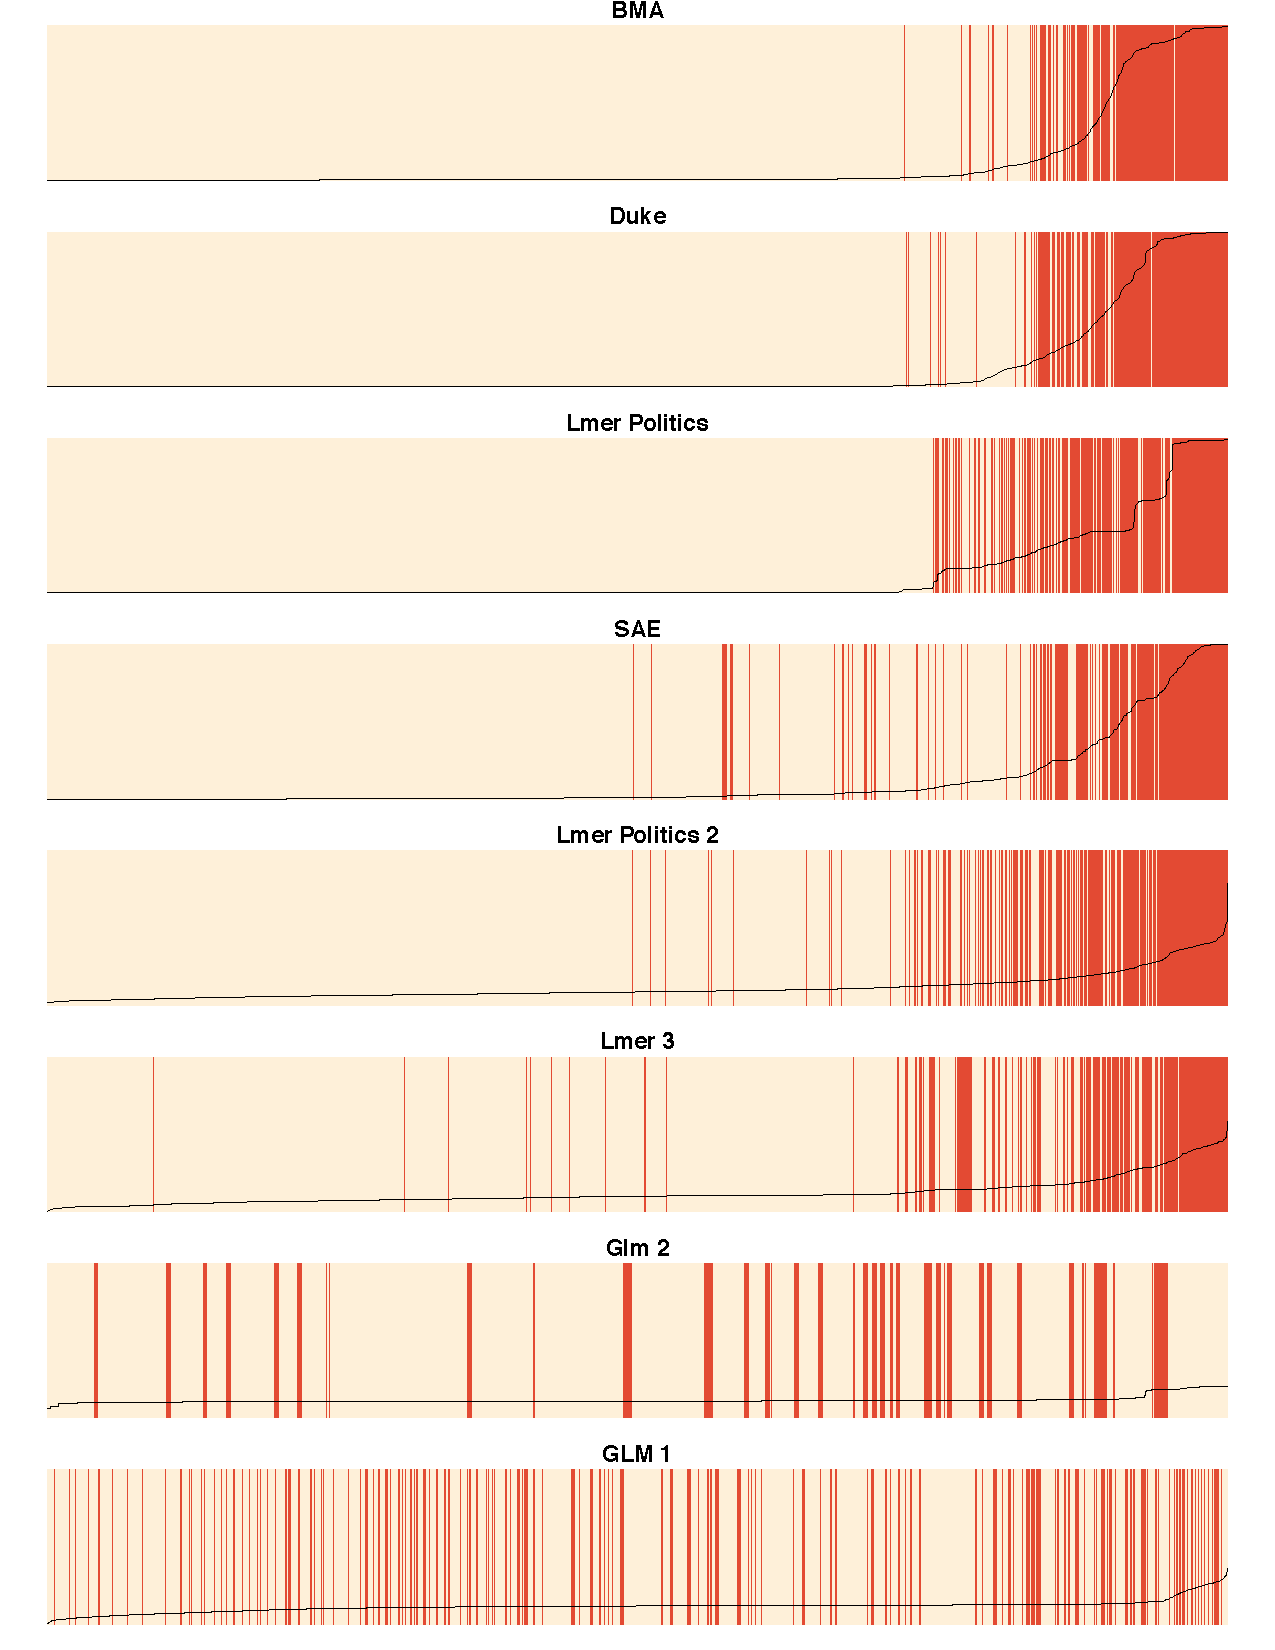
\includegraphics[width=6.2 in]{Plots_Insample}
\end{figure}

Figure \ref{InSam2sep} shows the separation plots for the EBMA model
and its components for the predictions on the in-sample data. Again
the models are ordered with the largest AUC first and the smallest AUC
last. It is easy to see that the EBMA model is very similar to the Duke
component, which by far has the highest weight. Both the EBMA and Duke
model make very accurate predictions, whereas the Lmer Politics 1 and
SAE components have more false negatives than the other two models. Again,
not surprisingly, the two simple GLM components are performing the worst.

Testing the seven individual components and the EBMA model on the
out-of-sample data set leads to similar results. Because of the high
weight associated with the Duke component, the results from the EBMA process are
almost indistinguishable from the Duke model output. Table \ref{OutSam2}
shows the results from the out-of-sample test of each of the components
and the EBMA model, which here includes the Duke model.

% latex table generated in R 2.11.1 by xtable 1.5-6 package
% Sun Mar  6 17:45:55 2011
\begin{table}[ht]
\begin{center}
\caption{model statistics -- out-of-sample predictions with the
Duke model}
\label{OutSam2}
\begin{tabular}{rrrrr}
  \hline
 & AUC & PRE & Brier & \% Correct \\ 
  \hline
Lmer Politics & 0.94 & 0.05 & 0.06 & 89.94 \\ 
  Glm 1 & 0.72 & 0.00 & 0.09 & 89.37 \\ 
  Lmer Politics 2 & 0.97 & 0.00 & 0.07 & 89.37 \\ 
  Glm 2  & 0.84 & 0.00 & 0.09 & 89.37 \\ 
  Lmer 3 & 0.97 & 0.00 & 0.07 & 89.37 \\ 
  Duke & 0.97 & 0.12 & 0.07 & 90.66 \\ 
  SAE & 0.96 & 0.04 & 0.06 & 89.80 \\ 
  BMA & 0.97 & 0.12 & 0.07 & 90.66 \\ 
   \hline
\end{tabular}
\end{center}
\end{table}

The out-of-sample predictions of the EBMA model are roughly equivalent
to the Duke component. Furthermore, given the small number of actual
occurrences in the data and the high number of correctly predicted
insurgencies in the Duke model, it is almost impossible to improve the
forecast through EBMA.  However, the EBMA model certainly does no worse
than any of individual model and, in fact, does slightly better by
some metrics.

\begin{figure}[ht!]
\caption{separation plots -- out-of-sample prediction with the
Duke model}
\label{OutSam2sep}
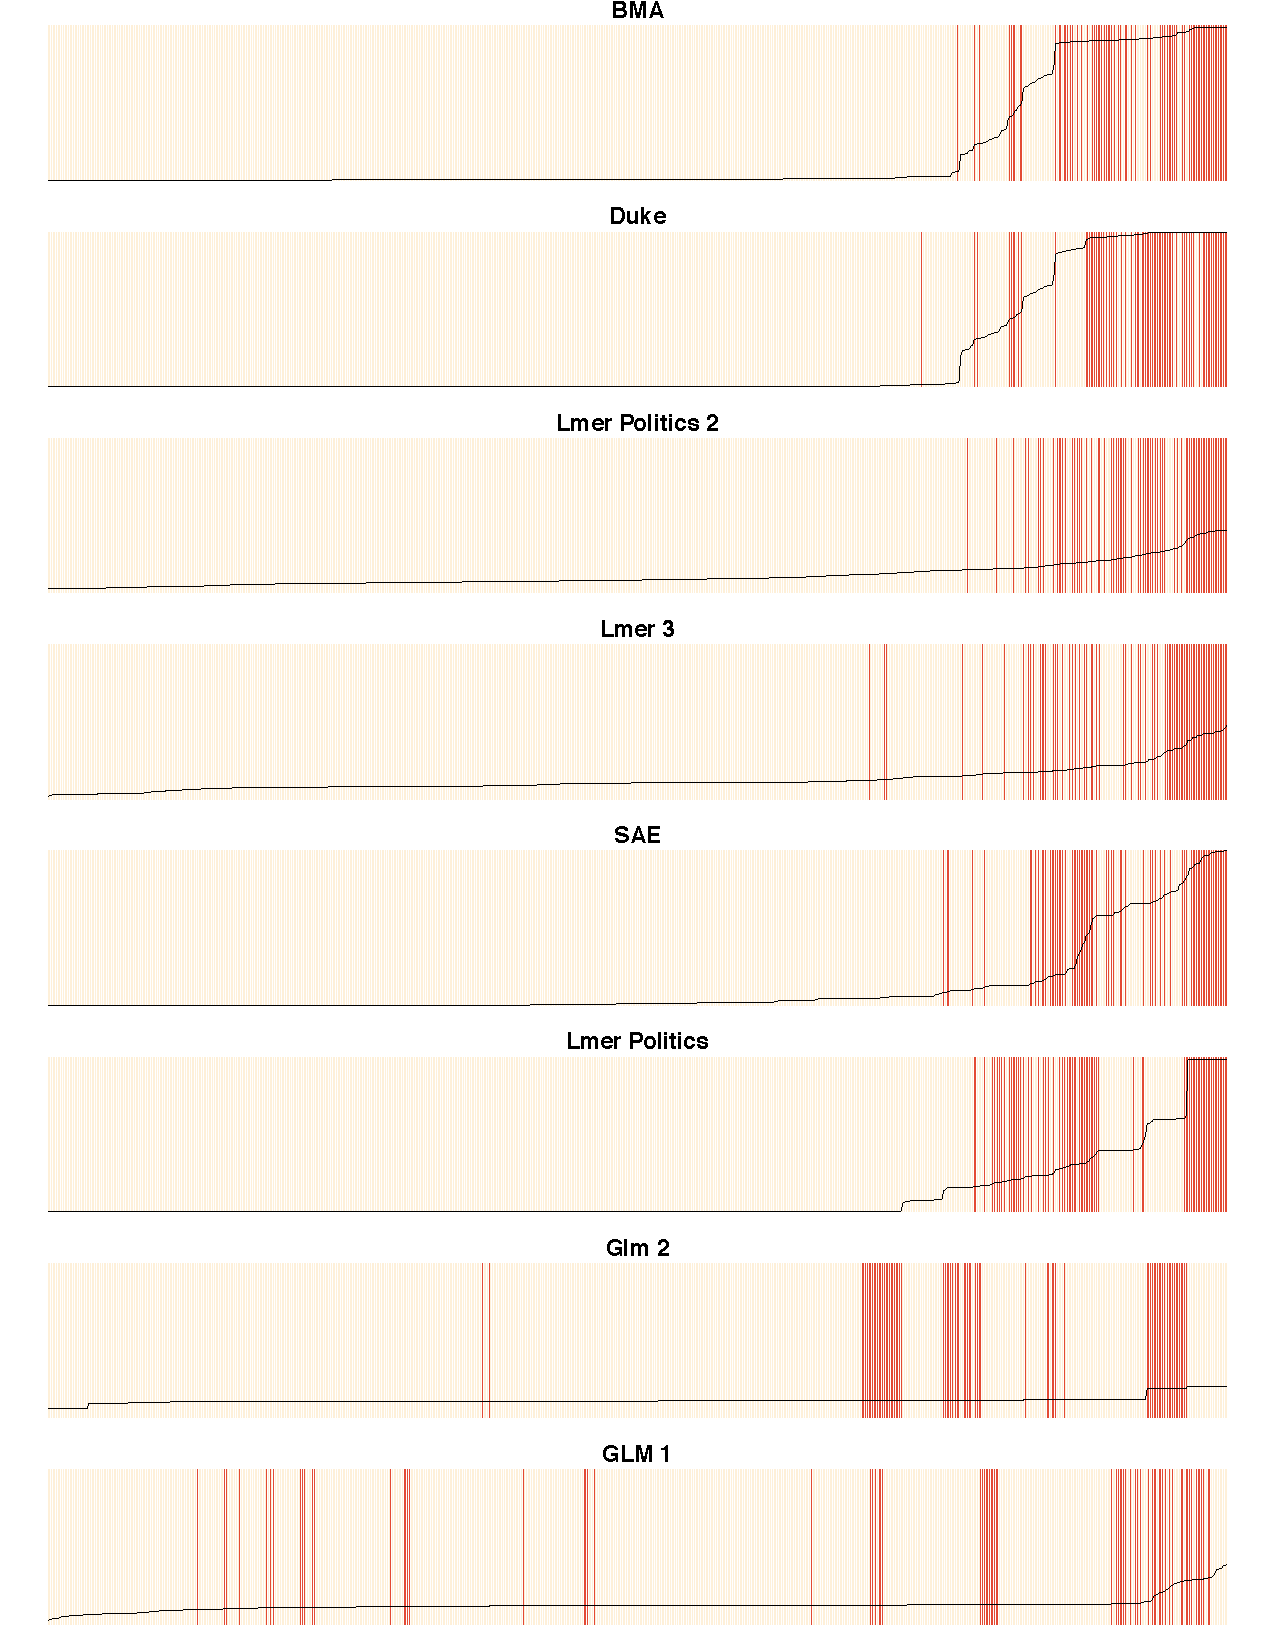
\includegraphics[width=6.2 in]{Plots_Outsample}
\end{figure}

Figure \ref{OutSam2sep} shows the separation plots of the EBMA model
and its components.  While the EBMA model obviously
is very similar to the Duke model, one can see that the EBMA model
performs slightly better and has considerable higher predicted
probabilities for observations with actual events.  However, as
emphasized above, it is nearly impossible to improve the forecast by
the Duke component on this data set by combining it with any other
individual model. Thus even the slight improvement that is achieved
here by the EBMA model shows the promise of the EBMA
process in improving the accuracy of out-of-sample forecasts.

\section{Discussion}

In many areas, political scientists rarely make predictions about the
future. To a large part this is due to the fact that it is almost
impossible to find the true data generating process of events that are
interesting to political science. Social events are inherently
difficult to predict because of nonlinearities and the
``unpredictability'' of human behavior. Yet, we believe it should be
the ultimate goal of political scientists to make sensible and
reliable predictions into the future.

In this paper, we extended previous work on Ensemble Bayesian Model
Averaging (EBMA) to make the technique applicable to binary dependent
variables. In short, EBMA uses the accuracy of in-sample predictions
of individual models to combine the power of multiple forecasts and
make more accurate predictions for future events.  Moreover, it does
so in a transparent manner that allows us to see which component
models are most important in informing the broader EBMA model.  Thus,
EBMA can help us to make reliable forecasts in political science more
likely, while also allowing the continued development of multiple
theoretical and empirical approaches to study important topics. In
this paper we have shown how the method can be adjusted to work for
dichotomous dependent variable.  The EBMA model developed here, based
on previous work \citet{Sloughter:2007} and \citet{Sloughter:2010}, is
thus applicable to a large fraction of research in political science,
but the field of international relations in particular. 

We have then shown the contribution of using EBMA to produce out-of-sample forecasts. Using six to seven individual models on the EBMA
process and comparing the predictions of the individual components to the
predictions of a final EBMA model, we were able to show that the
method improves the accuracy of predictions considerably. Even though
insurgency is an extremely rare even in our example data and improvements
of predictions from the individual models are thus difficult to
achieve, the EBMA predictions are always better or at least as good as any
of the individual components. Given the difficulty associated with this
particular dataset, the improvements of EBMA should be even more
distinct when applied to other settings and tested on other
datasets. In future versions of this paper we will provide more tests
to the superiority of EBMA compared to individual models forecasts.
Given the applicability of the framework to event data, one can also use
EBMA to increase the accuracy of predicting rare conflictual events
such as  civil war, revolutions, international conflict.

An additional planned extension of the EBMA method will be greater
inclusions of the uncertainty in component estimates in the final
ensemble predictions.  We anticipate that this may aid us
to even further increase the improvement of forecasts achieved by EBMA
as this information is currently lost through the sole reliance on
point predictions from the component models.  



\singlespacing

%\appendix
%\section*{Data Appendix} % Parts can probably be taken from the APSA
%paper YES ALL OF IT 

 \bibliographystyle{apsr}
\bibliography{Flo_Bib,/Users/jacobmontgomery/Dissertation/master3}
%\bibliography{/Users/mw160/Documents/BIBTEXFILES/predictionrefs/predictions2,/Users/mw160/Documents/BIBTEXFILES/2009mdwbib}}

\newpage

Contact information for authors:

\end{document}
\bye
